\documentclass[../thesis.tex]{subfiles}
\begin{document}
\chapter{Background}
\label{ch:background}

Generating token predictions for network configurations requires knowledge from multiple domains. In this section, we introduce router configurations and the tools available for writing as well as managing them. We also expand on some code completion techniques that have been successful for programming languages and form a basis for our engine.

\section{Network Configurations} 

Router configuration files are often written in a vendor specific language, the popular ones being provided by Cisco and Juniper systems. These files often exist as plain text on the routers and are composed of different types of `stanzas'. A stanza is defined as the largest contiguous block of commands that encapsulate a piece of the router's functionality. The most important types of stanzas include routing protocol, access-control list (ACL), and interface. Each stanza describes the router's particular role in relation to the stanza type. Network operators will configure these stanzas to define how the routers interact with each other. For example, operators might specify which devices the given router is connected to and what protocol it should follow when communicating with such devices. Additionally, they could enforce security measures by using access-control lists to block certain hosts from entering or leaving a network.\\

 Consider the configuration file for the router with hostname A in Figure 2.1. We can see an ACL stanza near the top which is configured to deny communication from any IP address beginning with 12. A few interface stanzas follow right below it, which define how this router is connected to other routers with some details about the connections (such as costs associated with using those routes). Lastly, at the bottom, we see a routing protocol stanza which states that the router uses the OSPF protocol to connect to two subnets. Here we can see some inklings of general purpose programming languages. We have certain keywords to set parameters (such as cost) for stanzas and define particular aspects of the router. We also have some notion of variables, where we can reuse predefined values. For example the last line in the first interface stanza, we use the access list with ID 1 that was defined in the ACL stanza above it. The similarities with programming languages that we observe motivate us to consider code completion techniques to help guide the development of our engine.

\begin{figure}[H]
	\centering
	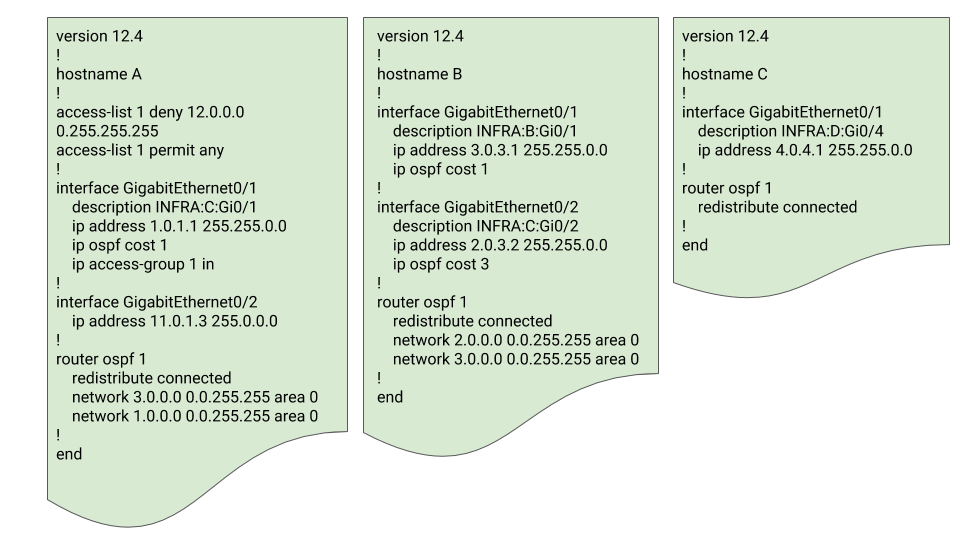
\includegraphics[width=5in]{configs-redone.png}
	\caption{A set of simplified configurations for a small network with four routers employing a single OSPF protocol.}
\end{figure}

\section{Code Completion}

Traditional completion techniques, such as those seen in IDEs~\cite{intelliJ-completion}, generate context-aware models of program histories. This means the code completion engines have to be aware of the grammar of the programming language and make suggestions based off that. Additionally, they maintain a record of past objects, their types and method calls invoked on them. If the user starts typing code with a similar type structure, they use this model to generate and rank the suggestions. These solutions offer fairly respectable accuracies but come with their idiosyncrasies. Popular IDEs, such as IntelliJ~\cite{intelliJ} or Eclipse~\cite{eclipse}, use relatively simple type based inferential techniques to suggest all methods available for an object, usually sorted in alphabetical order. Researchers, on the other hand, have proposed more ‘intelligent’ forms of code completion techniques in the past. Early work started by adopting rule based approaches where a database of predefined rules could be continuously queried to carry out possible completion tasks~\cite{kaiser}.  Other researchers explored how to make use of program history to offer suggestions based on what users had done in the past~\cite{robbes}.\\  

Eventually people started applying machine learning techniques, such as K-Nearest Neighbours, to extract patterns from existing code bases and building models that could be used to rank possible predictions for a given input vector~\cite{bruch}. All these techniques, however, require some form of context extraction, so that information about the codebase can be stored e.g. in form of a feature vector. They heavily leverage the existing code structure and require knowledge about the grammar of the programming language. A similar methodology for network configurations would require carefully extracting information from the parse-tree to ensure that the context of the tokens was properly understood. We go into a little more detail about some code completion techniques in Section 5.2.\\

Natural Language Processing (NLP) techniques, on the other hand, can generate predictions based on token usage and do not need to be explicitly aware of the grammar. This allows us to use these techniques independent of vendor specific configuration languages. Our inspiration for using NLP techniques primarily came through Hindle,\textit{et al.} 2012 ~\cite{naturalness}. This paper provides an excellent insight into the regularity of software code. The authors draw parallels between natural languages and codebases, and show that software is just as predictable as many human languages. They used an n-gram model to demonstrate high regularity in a dataset of Java projects, compared to an English corpus. They also proved that these results arose directly from the ‘natural’ regularity of the codebases rather than being an artefact of the programming language being syntactically simpler than English. Similar to Hindle,\textit{et al.}, Raychev \textit{et al.} 2015~\cite{raychev} took an NLP inspired an approach to generating code completions. They reduced the problem to predicting probabilities of sentences, performing static analysis on the code and feeding the results to two statistical language models: N-gram and Recurrent Neural Networks (RNN). They collect a history of method calls and treat them as sentences to synthesize suggestions. Interestingly, using RNNs had a negligible effect on their accuracies even though it increased the training time by many folds. Consequently, we have decided to use N-gram models as they seemed to work surprisingly well for both Raychev \textit{et al.} and Hindle,\textit{et al.}. We detail this model in Section 3.

\section{Network Management Tools}

It is important for us to recognize existing tools for managing networks and their shortcomings. One of the main motivations for pursuing this research is the lack of resources available for network operators to write configurations. Most routers offer some form of simple built-in Command Line Interface (CLI), where operators can use vendor specific languages to update router configurations. Often, these CLIs will offer rudimentary tab completion, where they will alphabetically suggest all the options available for a token from the invocation point. These are sometimes unhelpful as the user then has to search for the desired completion.\\ 

Enterprise network management tools, on the other hand, are built to assist network operators as they design, maintain and monitor large sets of router configurations. These tools often also offer various functionality to help write router configurations. NetMRI~\cite{netmri}, for example, allows users to use existing templates or write their own scripts to automate simple changes across the network. These changes might include adding ACLs, updating the router OS etc. SolarWinds~\cite{solarwinds}, a similar product, claims to simplify and standardize complex configuration changes by creating a single vendor-neutral script that can be scheduled and executed on multiple devices.\\

A recurring drawback of these tools is that they focus mostly on updating existing configurations. They do not provide any additional functionality for writing new configurations other than utilizing templates. Even in the latter case, the operators will have to fill in the templates appropriately or write their own custom templates for specialized router roles. Our work acknowledges that in practice no network’s functionality can be captured by templates alone. Thus, there is a need for an engine that can distinguish itself from these existing tools by being agnostic towards where it is used in the network development life cycle. We expect our engine to perform consistently whether invoked while writing new configurations or updating existing ones.


\end{document}
